\chapter{Okosotthon bemutatása és felépítése}

Az intelligens otthon a számítógépes technológiát, a vezérlési technológiát, a képmegjelenítési technológiát és a kommunikációs technológiát különböző hálózatán keresztül összekapcsolják, hogy megfeleljen a
az egész rendszer automatizálási követelményeinek teljesítése érdekében, hogy kényelmesebb vezérlést és irányítást biztosítson. Az intelligens otthon nagyjából a következőképpen írható le,
egy lakás, ahol rendszerint megtalálhatóak intelligens eszközök, amely rész egy otthoni belső
hálózatnak lehetővé téve az információk továbbítását
az eszközök között, és egy, az okosotthonokat összekötő lakossági átjáró, ami összeköti az otthont és a külső internetes világot. Ezek az eszközök, tárgyak
lehetővé teszik a tulajdonos számára, hogy interakcióba léphessenek velük, illetve lehetőség van az adatok tárolására, további viselkedési minták kialakításához.
\par Egy intelligens hálózat egyik legfontosabb alkotó eleme 
a távközlés. A távközlési rendszerek lehetővé teszik, hogy összeköttetésben legyenek az okosotthonban lévő eszközeink és ha igény van rá ellenőrizni tudjuk azokat.
\begin{figure}[!ht]
    \centering
    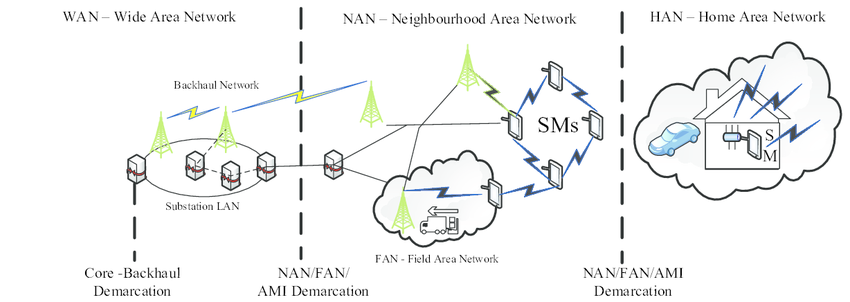
\includegraphics[width=70mm, keepaspectratio]{figures/han,nan,wan.png}
    \caption{Home area network (HAN), Neighborhood Area Network (NAN), Wide area network (WAN) }
\end{figure}
\newline A távközlési rendszerek a következőképpen csoportosíthatók
földrajzi terület szerint, ugyanazt a célt szolgálva:
\begin{itemize}
    \setlength\itemsep{-2pt}
    \item Home area network (HAN)
    \item Neighborhood Area Network (NAN)
    \item Wide area network (WAN)
\end{itemize}
\section{Intelligens otthoni rendszer modell}
Egy lakásba integrálható intelligens tárgyak lehetnek olyan egyszerűek, mint egy lámpa, amelyet távolról is vezérelhetünk vagy lekérdezhetjük a valós idejű állapotáról. Lehet például egy hűtőszekrény, amely tisztában van és tudja irányítani az állapotát és képes változtatni azt vagy akár egy otthon hagyott telefon is. Biztonsági rendszerek...stb.
\par Az otthoni hálózat a (HAN), 10\%-os átviteli sebességet igényel.
A hálózatnak 5 kbps és 1 Mbps közötti sebességet és 5 és 100 közötti távolságot kell lefednie.
Legfeljebb 5 méteres távolságot kell lefednie.

Minden eszköz csatlakozik az otthoni hálózathoz, hogy megadják az állapotukat, utasításokat kapjanak és vezérelhetőek legyen távolról. Az otthoni hálózat lehetővé teszi, hogy az otthon teljes mértékben összekapcsolódjon, mind külsőleg, mind belsőleg vezérelve. Az otthoni hálózati átjáró (gateaway) biztosítja a külső hozzáférést közvetlen kábelos interneteléréssel vagy az WiFi-n keresztül. Az átjáró lehetővé teszi az otthoni csatlakozást és az új szolgáltatások letöltését. A szolgáltató felelős az új szolgáltatásokért és azok elérhetőségéért a lakók számára.\cite{ricquebourg2006smart}
\begin{figure}[!ht]
    \centering
    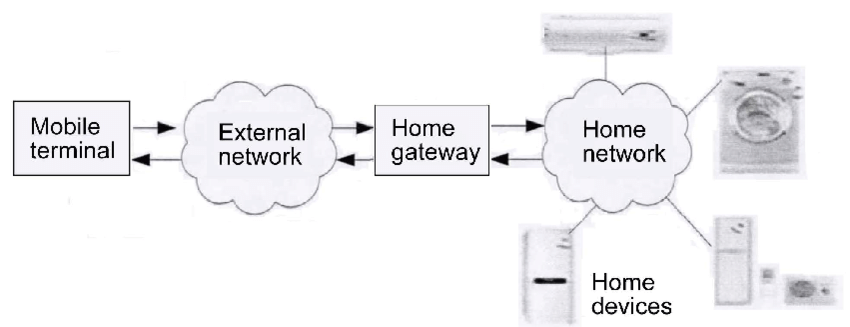
\includegraphics[width=70mm, keepaspectratio]{figures/Structure-of-smart-home-system.png}
    \caption{Okosotthoni rendszer felépítése}
\end{figure}

\section{IoT alapú intelligens otthon kialakítása}
Annak elérése érdekében, hogy minden eszköz kapcsolatban álljon egymással, valamilyen vezeték nélküli kommunikációs szabványt kell alkalmaznunk. A legelterjedtebb és legkönnyebben alkalmazható a Zigbee technológia ami alkalmas egy okosotthon felépítéséhez. Az eszközeink érzékeléséhez szükségünk lesz helyi otthoni hálózatra. Szükségünk van internetelérésre is, ami lehet ethernet vagy mobilinternet is. Ez teszi lehetővé hogy összekapcsolódjunk az internet világával. 
\par A rendszer három rétegre oszlik: érzékelő és működtető réteg, hálózati réteg és alkalmazási réteg.


\subsection{Mi is az a Zigbee?}
A Zigbee egy vezeték nélküli kommunikációs forma, amelynek az alapja az IEEE 802.15.4 hálózati szabvány és a személyi hálózatot használja. A 802.15.4 lehetővé teszi a hálózatok létrehozását 
peer-to-peer kapcsolódással és olyan hálózati topológiával, ahol nincsen központi csomópont, mint például a csillag és a hálós topológia. Hatósugara 10 métertől akár 300 méterig is terjedhet.
Kiváló példa a működésének bemutatásához, hogy amikor van egy intelligens izzó és egy villanykapcsoló, amit szeretnénk összekapcsolni, hogy a kapcsolóval tudjuk irányítani az izzót. A Zigbee kommunikáció segítségével a két eszközt össze tudjuk hangolni, hogy megértsék egymást, még akkor is, ha azok teljesen más gyártótól származnak.
\par A Zigbee-t erdetileg nem P2P kommunikációra tervezték, mint például a Bluetooth-t. Használatához mindenképpen szükség van egy helyben felszerelt központi egységre, egy hubra vagy átjáróra, amellyel lehetőség van arra, hogy minden eszköz tudjon egymással kapcsolatban lenni és kommunikálni.
A Zigbee további előnye, hogy egy tisztán Zigbee-alapú rendszerben csak a hub rendelkezik WiFi vagy vezetékes internetkapcsolattal. Mivel ezek az eszközök teljesen különböző frekvenciákat használnak így például az okostelefonok, melyek nem képzik az intelligens hálózatnak a részét nem terhelik túl a WiFit, így nem lassítva az interneten való böngészést a felhasználók számára.
\par Ez technológia több mint egy évtizede jelen van a piacon és sokan a Wi-Fi és a Bluetooth technológia alternatívájaként tekintik. Alacsony energiafogyasztása teljesen kompatibilis és optimális a nagy sávszélességet nem igénylő eszközökhöz.
Be kell vallani, hogy a Zigbee igénytelen, egyszerű, viszont megbízható és kiválóan működik, ha intelligens rendszer kialakítása érdekében szeretnénk összekötni eszközeinket.\cite{4127535}

\subsubsection{}
